\documentclass[Lecture.tex]{subfiles}
\begin{document}
\section{4.1: Displaying Relationships Between Categorical Variables}

\begin{frame}{Think-Pair-Share}
Hair color and eye color are related characteristics.  What exactly does it mean to say that these two variables are related?  Suppose you know the hair colors and eye colors of 200 individuals.  How would you assess whether the two variables are related for those individuals?
\end{frame}

\begin{frame}{Categorical Variables}
\begin{defn}
Recall that raw data from {\it categorical variables} consist of group or category names that don't necessarily have any ordering.
\end{defn}\pause
The principal question we ask in most cases is, ``Is there a relationship between the two variables such that the category into which individuals fall for one variable seems to depend on the category they are in for the other variable?"
\end{frame}

\begin{frame}{Displaying Relationships}
We have already seen an example of this type of problem:
\begin{center}
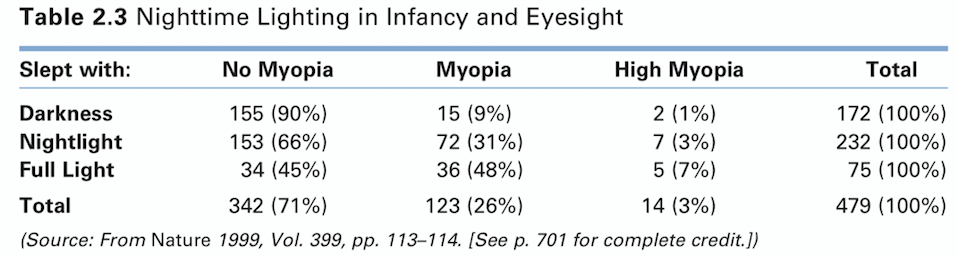
\includegraphics[scale=.3]{myopia}
\end{center}\pause
We can provide a clearer summary using the following bar chart.
\end{frame}
  
\begin{frame}{Contingency Table}
\begin{center}
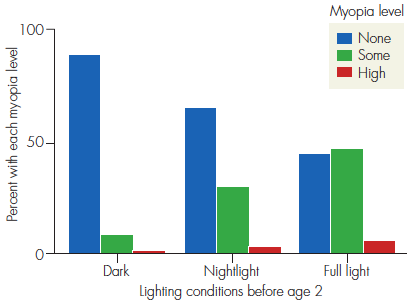
\includegraphics[scale=.4]{myopiabarchart}
\end{center}\pause
\begin{defn}
The type of display above is also call a {\it contingency table} because it covers all contingencies for the combinations of the two variables.  They are also sometimes referred to as {\it two-way tables}.\pause Each row category and column category combination in the table is called a {\it cell}.
\end{defn}
\end{frame}

\begin{frame}{Summary}
\begin{itemize}
\item<1->
A {\it row percentage} uses a total row count as the basis for computing a percentage.  It is the percentage of the observations within a particular row category that are in a specified category of the column variable. (See the myopia example.)
\item<2->
A {\it column percentage} uses a total column count as the basis for computing a percentage.
\item<3->
There is a {\it relationship} between the categorical variables that form a two-way table if two or more rows (columns) have different distributions of row (column) percentages.
\end{itemize}
\end{frame}  
  
  

  
  
  
  
  
  
  
  
  
  
  
  
  
  
  
  
\end{document}
